\documentclass[landscape,a0paper,fontscale=0.33]{baposter} % Adjust the font scale/size here
\usepackage{graphicx} % Required for including images
\graphicspath{{figures/}} % Directory in which figures are stored
\usepackage{amsmath} % For typesetting math
\usepackage{amssymb} % Adds new symbols to be used in math mode
\usepackage[pdftex]{color}
\usepackage{booktabs} % Top and bottom rules for tables
\usepackage{enumitem} % Used to reduce itemize/enumerate spacing
\usepackage{palatino} % Use the Palatino font
\usepackage[font=small,labelfont=bf]{caption} % Required for specifying captions to tables and figures
\usepackage{multicol} % Required for multiple columns
\setlength{\columnsep}{1.5em} % Slightly increase the space between columns
\setlength{\columnseprule}{0mm} % No horizontal rule between columns

\usepackage{tikz} % Required for flow chart
\usetikzlibrary{shapes,arrows} % Tikz libraries required for the flow chart in the template

\newcommand{\compresslist}{ % Define a command to reduce spacing within itemize/enumerate environments, this is used right after \begin{itemize} or \begin{enumerate}
\setlength{\itemsep}{1pt}
\setlength{\parskip}{0pt}
\setlength{\parsep}{0pt}
}

\definecolor{lightblue}{rgb}{0.145,0.6666,1} % Defines the color used for content box headers
\definecolor{red}{rgb}{1,0,0}
\definecolor{blue}{rgb}{0,0,1}
\definecolor{lila}{rgb}{1,0,1}
\definecolor{brightgreen}{rgb}{0.4, 1.0, 0.0}

\begin{document}

\begin{poster}
{
headerborder=closed, % Adds a border around the header of content boxes
colspacing=0.5em, % Column spacing
bgColorOne=white, % Background color for the gradient on the left side of the poster
bgColorTwo=white, % Background color for the gradient on the right side of the poster
borderColor=lightblue, % Border color
headerColorOne=black, % Background color for the header in the content boxes (left side)
headerColorTwo=lightblue, % Background color for the header in the content boxes (right side)
headerFontColor=white, % Text color for the header text in the content boxes
boxColorOne=white, % Background color of the content boxes
textborder=roundedleft, % Format of the border around content boxes, can be: none, bars, coils, triangles, rectangle, rounded, roundedsmall, roundedright or faded
eyecatcher=true, % Set to false for ignoring the left logo in the title and move the title left
headerheight=0.1\textheight, % Height of the header
headershape=roundedright, % Specify the rounded corner in the content box headers, can be: rectangle, small-rounded, roundedright, roundedleft or rounded
headerfont=\Large\bf\textsc, % Large, bold and sans serif font in the headers of content boxes
%textfont={\setlength{\parindent}{1.5em}}, % Uncomment for paragraph indentation
linewidth=2pt % Width of the border lines around content boxes
}
%----------------------------------------------------------------------------------------
%	TITLE SECTION 
%----------------------------------------------------------------------------------------
%
{\includegraphics[height=7.5em]{LogoUC.png}} % First university/lab logo on the left
{\bf\textsc{Regional contributions of ocean iron fertilization to atmospheric $CO_2$ changes during the
last glacial termination}} % Poster title
{\textsc{Natalia Opazo, Fabrice Lambert \\
\hspace{12pt} Pontifical Catholic University of Chile}}% Author names and institution
{\includegraphics[height=5em]{DICE.png}} % Second university/lab logo on the right


%	INTRODUCTION
%----------------------------------------------------------------------------------------

\headerbox{Introduction}{name=introduction,column=0,row=0}{

Oceans are the largest source of carbon storage. Their internal processes directly affect the concentrations of atmospheric $pCO_2$. In the last 2 million years the climate of the Earth
has alternated between glacial and interglacial periods, with low and high atmospheric concentrations of $CO_2$. Iron fertilization of the oceans is though to have contributed a
pproximately 20 p.p.m.v. to the 80-100 p.p.m.v. Holocene-LGM difference in atmospheric $CO_2$ concentrations

\begin{center}
\includegraphics[width=0.8\linewidth]{bomba.png}
\captionof{figure}{A schematic of the ocean's ``biological pump``, the sequestration of carbon and alkalinity from the surface ocean (light blue) into the ocean
interior (dark blue), and their effects on the ocean's carbon chemistry. Source \cite{Hain2014}.}
\end{center}

In this study, we explore the effect of iron fertilization through mineral dust flux to the ocean surface for Holocene and LGM climatic conditions, but also for idealized intermediate
dust values. In this way, we can calculate the theoretical relationship between dust fluxes and atmospheric pCO2 through the modulation of the biological pump in the ocean ({\bf Figure 1}).}

\headerbox{ Materials and Methods}{name=Materials and Methods,column=1,row=0,bottomaligned=introduction}{

We use the cGENIE carbon cycle-focused Earth System Model of Intermediate Complexity to simulate the effect of various dust fields on atmospheric CO2 through the termination.
For five different published Holocene and LGM dust flux estimates \cite{Lambert2015,Albani2014,Takemura2009,Watanabe2011,Yukimoto2012}. 

\begin{center}
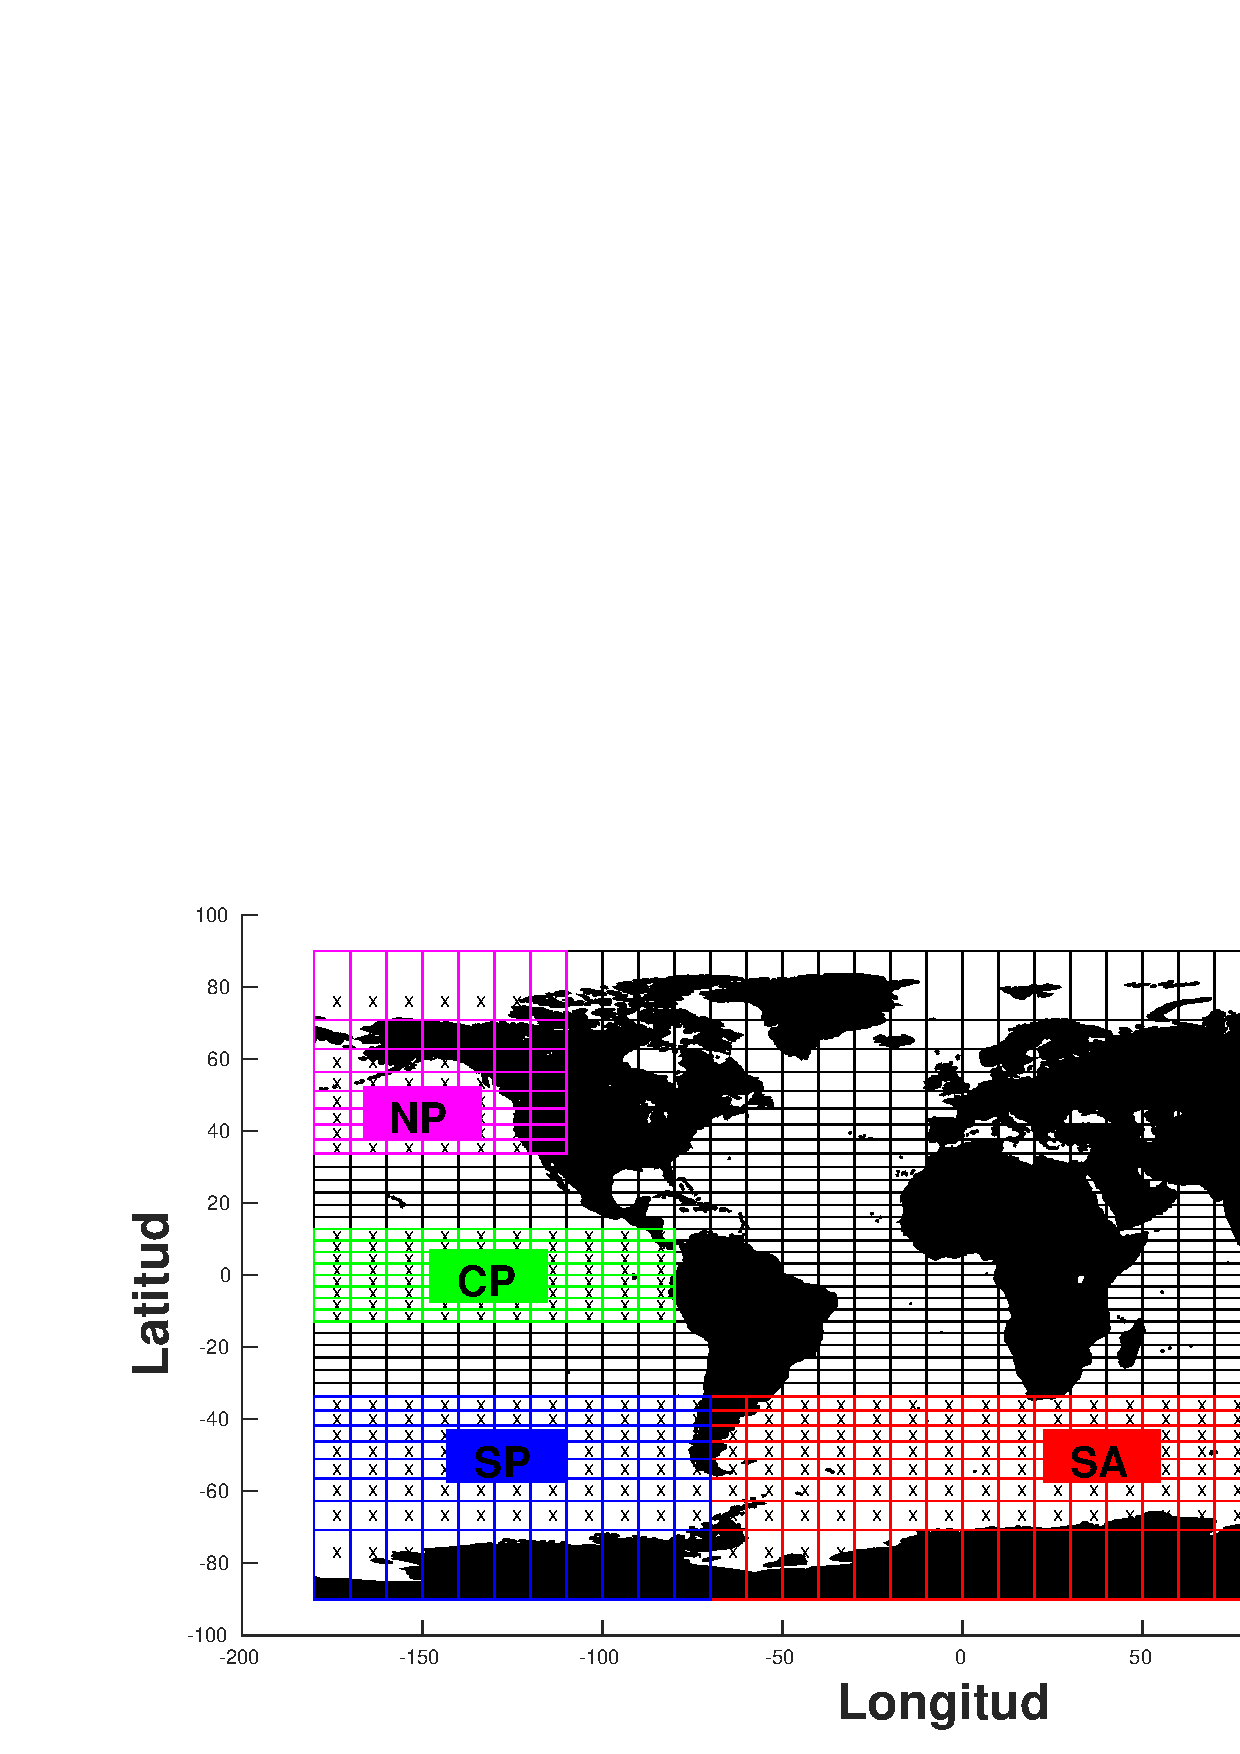
\includegraphics[width=1\linewidth]{mapa.png}
\captionof{figure}{Grid with the specification of oceanic regions run with cGENIE}
\end{center}

We produced 8 linearly-spaced intermediate dust flux values at each grid point, thus resulting in 10 incremental global dust flux fields from low Holocene to high LGM values.
We simulate the response of atmospheric CO2 through the termination for global dust fluxes, but also isolate specific High-Nutrient Low Chlorophyll (HNLC) regions of the world's ocean 
(Figure 2) to quantify their individual contribution to the total CO2 changes.
}


\headerbox{$\begin{array}{l}\vspace{-1cm}\\
{$pCO_2$ reduction obtained by cGENIE simulation for dust fields}\\ \text{ varying from Holocene to LGM}
\end{array}$
}{name=results,boxheaderheight=1.1cm,column=2,span=2,row=0}{
%\headerbox{$pCO_2$ reduction obtained by cGENIE model for dust fields}{varying from Holocene to LGM}{name=results,boxheaderheight=2cm,column=2,span=2,row=0}{

\begin{multicols}{2}

\setlength{\fboxrule}{2pt}
\begin{center}
\includegraphics[width=1\linewidth]{R_All.png}
\captionof{figure}{Global fluxes.}
\end{center}

\setlength{\fboxrule}{2pt}
\begin{center}
\fcolorbox{lila}{white}{\includegraphics[width=0.93\linewidth]{PN.png}}
\captionof{figure}{North Pacific regional zone.}
\end{center}

\end{multicols}
\begin{multicols}{3}

 \begin{center}
\fcolorbox{brightgreen}{white}{\includegraphics[width=1\linewidth]{PC.png}}
\captionof{figure}{Central Pacific regional zone.}
\end{center}

 \begin{center}
\fcolorbox{blue}{white}{\includegraphics[width=1\linewidth]{PS.png}}
\captionof{figure}{South Pacific regional zone.}
\end{center}

\vspace{1cm}
 \begin{center}
\fcolorbox{red}{white}{\includegraphics[width=0.98\linewidth]{AS.png}}
\captionof{figure}{South Atlantic regional zone.}
\end{center}

\end{multicols}
}
\headerbox{Results}{name=results2,column=0,below=introduction,span=2,above=bottom}{

\begin{multicols}{2}
\vspace{1em}

\begin{center}
\includegraphics[width=1.25\linewidth]{R_final.png}
\captionof{figure}{Range percentage of $pCO_2$ reduction of models: Lambert, Albani, Takemura, MIROC-ESM, MRI-CGCM3. }
\end{center}

 \begin{center}
\includegraphics[width=0.66\linewidth]{Final_All_Puntos.png}
\captionof{figure}{Results cGENIE, a) range percentage of $pCO_2$ reduction for global dust fluxes and, b) contribution of each HNLC region to global LGM to Holocene $pCO_2$ reduction.}
\end{center}
\end{multicols}

}

\headerbox{Conclusion}{name=conclusion,column=2,below=results}{
\vspace{0.1cm}
There are only small changes in relative CO2 capture simulated by cGENIE due to different reconstruction or simulations of dust fluxes, both globally and regionally (Fig. 8 and 9a).
Note that this small error is largely due to our removal of those model results that did not change southern hemisphere dust source emissions between Holocene and LGM.\\

The high-latitude oceans contribute most to CO2-drawdown during the LGM (Fig. 9b). This was expected since they are the main HNLC regions of the world's ocean and therefore very
sensitive to the contribution of aeolian iron flux that influence on ocean biogeochemistry.
\vspace{0.4cm}
}
\headerbox{References}{name=references,column=3,below=results,above=bottom}{
{\setlength{\parskip}{0.3mm}
\renewcommand{\section}[2]{\vskip 0.05em} % Get rid of the default "References" section title
\nocite{*} % Insert publications even if they are not cited in the poster
\scriptsize{ % Reduce the font size in this block
\bibliographystyle{unsrt}
\bibliography{sample} % Use sample.bib as the bibliography file
}}}

\headerbox{Contact Information}{name=contact,column=2,below=conclusion,above=bottom}{ % This block is as tall as the references block

\begin{description}\compresslist
%\item[Web] www.university.edu/smithlab
\small{
\item[Email] neopazo@uc.cl}
\item[Email2] lambert@uc.cl
%\item[Phone] +56 (9) 56550788
\end{description}
}

\end{poster}

\end{document}
